\subsection{Theories with a rank-3 antisymmetric hypermultiplet}\label{}
Another non-trivial test of our blowup formula is the partition for 5d $SU(6)$ theory with an hypermultiplet in the rank-3 antisymmetric representation ({\bf TAS}), 
as it is a non-trivial calculation and the theory allows an intriguing Higgs branch which can be explicitly checked via the partition function.

To have UV fixed point, 5d $SU(6)$ theories can have up to 4 half-hypermultiplets in the rank-3 antisymmetric representation \cite{Jefferson:2017ahm}. Their Type IIB 5-brane configurations are also constructed in~\cite{Hayashi:2019yxj} with/without O5-planes. In particular, 5-brane web diagrams for $SU(6)+\frac12{\bf TAS}$ and $SU(6)+1{\bf TAS}$ do not require orientifold planes, so that topological vertex method \cite{Aganagic:2003db, Iqbal:2007ii} can be straightforwardly applicable to compute the partition functions. For instance, the partition function for $SU(6)_\frac52$ theory with one half-hypermultiplet in the rank-3 antisymmetric representation was computed up to two instantons \cite{Hayashi:2019yxj} using the topological vertex.
%---------  <Figure>  ---------------%
\begin{figure}[t]
\centering
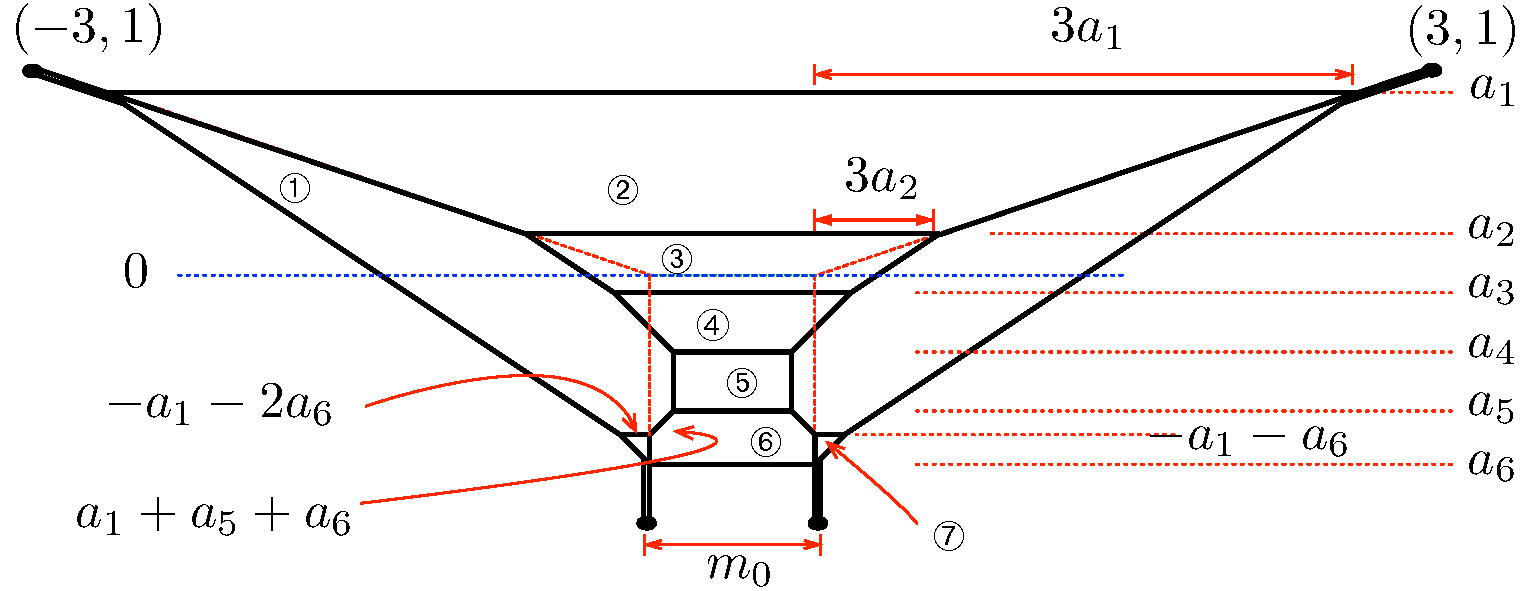
\includegraphics[width=12cm]{SU6-monopole.pdf}
\caption{A 5-brane web for $SU(6)_3$ theory with one massless hypermultiplet in the rank-3 antisymmetric representation.}
\label{fig:SU6-monopole}
\end{figure}
%----------- </Figure> ---------------%

To test our blowup formula, we need mass parameter for rank-3 antisymmetric hyper. As one cannot introduce mass for a half-hypermultiplet, we consider $SU(6)_3$ theory with one hypermultiplet (or two half-hypers) in the rank-3 antisymmetric representation ($SU(6)+1{\bf TAS}$). An example for 5-brane brane web for $SU(6)+1{\bf TAS}$ is depicted in Figure \ref{fig:SU6-monopole}. It is instructive to see that the 5-brane web given in Figure \ref{fig:SU6-monopole} is consistent with the prepotential for $SU(6)_3+1{\bf TAS}$.  The effective prepotential on Coulomb branch of a 5d gauge theory with a gauge group $G$ and matter $f$ in a representation $R_f$ is given by ~\cite{Intriligator:1997pq}
\begin{align}
\mathcal{F}(\phi) = \frac{m_0}{2}h_{ij}\phi_i\phi_j + \frac{\kappa}{6}d_{ijk}\phi_i\phi_j\phi_k + \frac{1}{12}\left(\sum_{r\in\text{roots}}\left|r\cdot \phi\right|^3 - \sum_f\sum_{w \in R_f}\left|w\cdot \phi - m_f\right|^3\right). \label{prepotential}
\end{align}
Here, $m_0$ is the inverse of the gauge coupling squared, $\kappa$ is the Chern-Simons level and $m_f$ is a mass parameter for the matter $f$. $r$ is a root of the Lie algebra $\mathfrak{g}$ associated to $G$ and $w$ is a weight of the representation $R_f$ of $\mathfrak{g}$. We also defined $h_{ij} = \text{Tr}(T_iT_j), d_{ijk} = \frac{1}{2}\text{Tr}\left(T_i\{T_j, T_k\}\right)$ where $T_i$ are the Cartan generators of the Lie algebra $\mathfrak{g}$. With Coulomb branch moduli assigned in Figure \ref{fig:SU6-monopole} and the identification of Weyl chamber for the Coulomb VEV ($a_1\ge a_2\ge \cdots \ge a_{6}$, $\sum_{i=1}^{6}a_i=0$),
\begin{align}
	a_1= \phi_1,&& 
	a_2=\phi_2-\phi_1,&&
	a_3=\phi_3-\phi_2,&&
	a_4=\phi_4-\phi_3,&&
	a_5=\phi_5-\phi_4,&&
	a_6=-\phi_5, \label{orth2Dynkin}
\end{align}
one finds that the prepotential for $SU(6)_3$ with one massless rank-3 antisymmetry hyper takes the form
\begin{align}
	\mathcal{F}_{SU(6)_3+1{\bf TAS}}=&~m_0 \big( \phi _1^2+\phi _2^2+\phi _3^2+\phi _4^2+\phi _5^2-\phi _1 \phi _2-\phi _2 \phi _3-\phi _3 \phi _4-\phi _4
   \phi _5\big) \cr
   &+ \frac{\phi _1^3}{3}+\frac{4 \phi _2^3}{3}+\frac{4
   \phi _3^3}{3}+\frac{4 \phi_4^3}{3}+\frac{4 \phi_5^3}{3}+4\phi_1^2 \phi_2 -5 \phi_1\phi_2^2 -2\phi_1 \big(\phi_3^2+\phi_4^2+\phi_5^2\big) \cr
  & +\phi_2^2 \phi_3-2 \phi_2 \phi_3^2-\phi_3 \phi_4^2-\phi _4^2 \phi_5+2 \phi _1\phi _2 \phi _3 +2\phi_1\phi_3\phi_4+2\phi_1\phi_4\phi_5. \label{eq:prep+SU6-3}
\end{align}
%\begin{align}
%	\mathcal{F}_{SU(6)_3+1{\bf TAS}}=&\,m_0 \big( \phi _1^2+\phi _2^2+\phi _3^2+\phi _4^2+\phi _5^2-\phi _1 \phi _2-\phi _2 \phi _3-\phi _3 \phi _4-\phi _4
%   \phi _5\big) \cr
%   &+ \frac{\phi _1^3}{3}+4 \phi _2 \phi _1^2-5 \phi _2^2 \phi _1+2 \phi _2 \phi _3 \phi _1-2 \left(\phi
%   _3^2-\phi _4 \phi _3+\phi _4^2+\phi _5^2-\phi _4 \phi _5\right) \phi _1\cr
%  & +\frac{4 \phi _2^3}{3}+\frac{4
%   \phi _3^3}{3}+\frac{4 \phi _4^3}{3}+\frac{4 \phi _5^3}{3}-2 \phi _2 \phi _3^2-\phi _3 \phi _4^2+\phi
%   _2^2 \phi _3-\phi _4^2 \phi _5. \label{eq:prep+SU6-3}
%\end{align}
From which, one can easily obtain the monopole string tensions $T_i=\partial{\mathcal{F}}/\partial{\phi_i}$ as the areas of the compact faces of the 5-brane web 
\begin{align}
T_1=\textcircled{\scriptsize 1} + 2\times\textcircled{\scriptsize 2},  %\crcr
&& T_2=\textcircled{\scriptsize 3}, %\crcr
&&T_3=\textcircled{\scriptsize 4}, %\crcr
&&T_4=\textcircled{\scriptsize 5}, %\crcr
&&T_5=\textcircled{\scriptsize 6} 
	+ 2\times\textcircled{\scriptsize 7},
\end{align}
where the encircled numbers represent the area of apparent faces in Figure \ref{fig:SU6-monopole}.
One can then see that the 5-brane web given in Figure \ref{fig:SU6-monopole} is consistent with the prepotential for $SU(6)_3$ with one massless rank-3 antisymmetric hyper.

 %---- <Figure>  ---------------%
\begin{figure}[t]
\centering
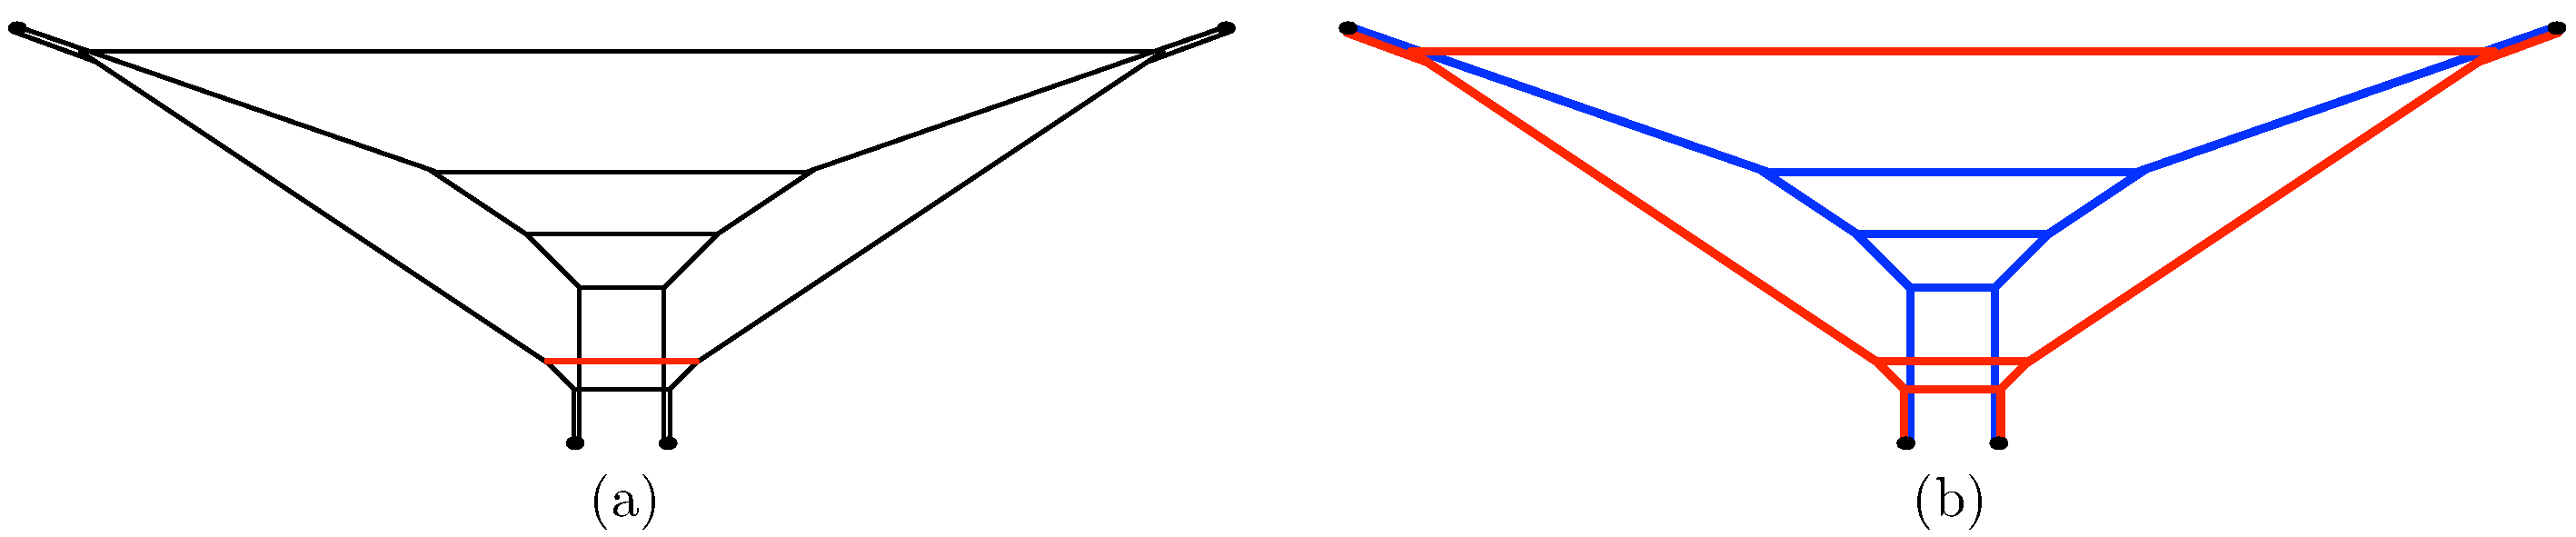
\includegraphics[width=12cm]{SU6-Higgsing.pdf}
\caption{(a) A Higgsing of $SU(6)_3+1{\bf TAS}$ into two $SU(3)_3$ theories by aligning internal D5-branes in red. (a) Two different $SU(3)_3$ theories are painted in blue and red, respectively. %As a result, a new Higgs branch emerges.
}
\label{fig:SU6-Higgsing}
\end{figure}
 %---- </Figure>  --------------%
 
Notice that this 5-brane web for $SU(6)_3+1{\bf TAS}$ suggests an intriguing Higgsing of the theory,  that is the Higgsing of $SU(6)$ theory with one rank-3 antisymmetric hyper into two pure $SU(3)$ theories. It can be achieved by setting the Coulomb branch parameters as
 \begin{align}
 	a_5= - a_1-a_6, \qquad {\rm or~equivalently} \qquad \phi_4=\phi_1. \label{eq:HiggisingToSU3}
 \end{align}
 This tuning of the parameters, of course, reduces the dimension of Coulomb brach  by one and also opens up a Higgs branch in such a way that the 5-brane web in Figure \ref{fig:SU6-monopole} becomes 5-brane web in Figure \ref{fig:SU6-Higgsing}(a) where the D5-branes in the upper parts of $\textcircled{\scriptsize 6}$ and $\textcircled{\scriptsize 7}$ are aligned and joint to become a single D5-brane that is paint in red in Figure~\ref{fig:SU6-Higgsing}(a). The resulting configuration is then a 5-brane configuration for two pure $SU(3)_3$ theories that are on top of each other, as shown in Figure~\ref{fig:SU6-Higgsing}(b). This Higgsing procedure is a 5-brane realization of the Higgsing of $SU(6)_3$ theory with a rank-3 antisymmetric hyper into two pure $SU(3)_3$ theories. It follows that 
 under this Higgsing, the prepotential for $SU(6)_3+1{\bf TAS}$ \eqref{eq:prep+SU6-3} becomes a sum of prepotentials for two independent pure $SU(3)_3$ theories (without bi-fundemantals):
\begin{align}
\mathcal{F}_{SU(6)_{3}+1{\bf TAS}}{}\Big|_{\phi_4=\phi_1}	&
\rightarrow \mathcal{F}_{SU(3)_{3}} (m_0, \phi_1, \phi_5-\phi_1,-\phi_5) + \mathcal{F}_{SU(3)_{3}} (m_0, \phi_2-\phi_1, \phi_3-\phi_2,\phi_1-\phi_3),\nonumber
\end{align}
or,
\begin{align}
\mathcal{F}_{SU(6)_{3}+1{\bf TAS}}{}\Big|_{a_1+a_5+a_6=0}	%\mathcal{F}(m_0,a_1,a_2,a_3,a_4,a_5,a_6)	
&\rightarrow \mathcal{F}_{SU(3)_3}(m_0,a_1,a_5,a_6)+\mathcal{F}_{SU(3)_3}(m_0,a_2,a_3,a_4).
\end{align}
The Higgsing of the $SU(6)$ theory into two copies of $SU(3)$ theories can be understood as follows. %Under the embedding
%\begin{align}
%	SU(6) \supset SU(3) \times SU(3) \times U(1),
%\end{align}
%Under this Higgsing, the hypermultiplet in the rank-3 antisymmetric representation and the gauge bosons transforming the adjoint of $SU(6)$ are decomposed as
%\begin{align}
%	SU(6) &\supset SU(3) \times  SU(3) \times U(1),\crcr
%%	
%	{\bf 20}&={\bf (1,1)}_3 + {\bf (1,1)}_{-3}+ {\bf (3,\bar3)}_{-1}+{\bf (\bar3, 3)}_{1}\crcr
%%	
%	{\bf 35 }& ={\bf (1,1)}_0 + {\bf (1,8)}_0 + {\bf (8,1)}_0 + {\bf (3,\bar3)}_2 +{\bf (\bar3, 3)}_{-2}.	
%\end{align}
This in turn implies that under this Higgsing, the partition function for $SU(6)_{3}+1{\bf TAS}$ should be expressed as a product of the partition functions of two pure $SU(3)_3$ theories  
\begin{align}
Z_{SU(6)_{3}+1{\bf TAS}}\big|_{\rm Higgsing}~\rightarrow ~~ Z_{SU(3)_{3}}\!(q,A_1, A_5,A_6)\,Z_{SU(3)_{3}}\!(q,A_2, A_3,A_4)\,Z_{\rm decoupled}(q)\,,	
\end{align}
%\begin{align}
%Z_{SU(6)_{3}+1{\bf TAS}}\bigg|_{\rm Higgsing}\qquad \rightarrow\qquad Z^{(1)}_{SU(3)_{3}}Z^{(2)}_{SU(3)_{3}}\,Z^{}_{\rm decoupled}\,,	
%\end{align}
%where 
%\begin{align}
%	Z^{(1)}_{SU(3)_{3}} &= Z_{SU(3)_{3}} (\phi_1, \phi_5-\phi_1,-\phi_5),\crcr
%	Z^{(2)}_{SU(3)_{3}} &= 	Z_{SU(3)_{3}}(\phi_2-\phi_1, \phi_3-\phi_2,\phi_1-\phi_3), 
%\end{align}
where the parameters $q$ and $A_i$ are the K\"ahler parameters for instanton and Coulomb branch parameters, and  $Z_{\rm decoupled}(q)$ represents the overall extra terms that do not explicitly depend on the Coulomb branch moduli, which would correspond to a new decoupled mode appearing in Figure \ref{fig:SU6-Higgsing}.  In what follows, we explicitly compute the partition function for $SU(6)_3+1{\bf TAS}$ based on the 5-brane web and compare it with our blowup formula, and also consider this Higgsing as a consistency check.

%---------  Figure  ---------------%
\begin{figure}[t]
\centering
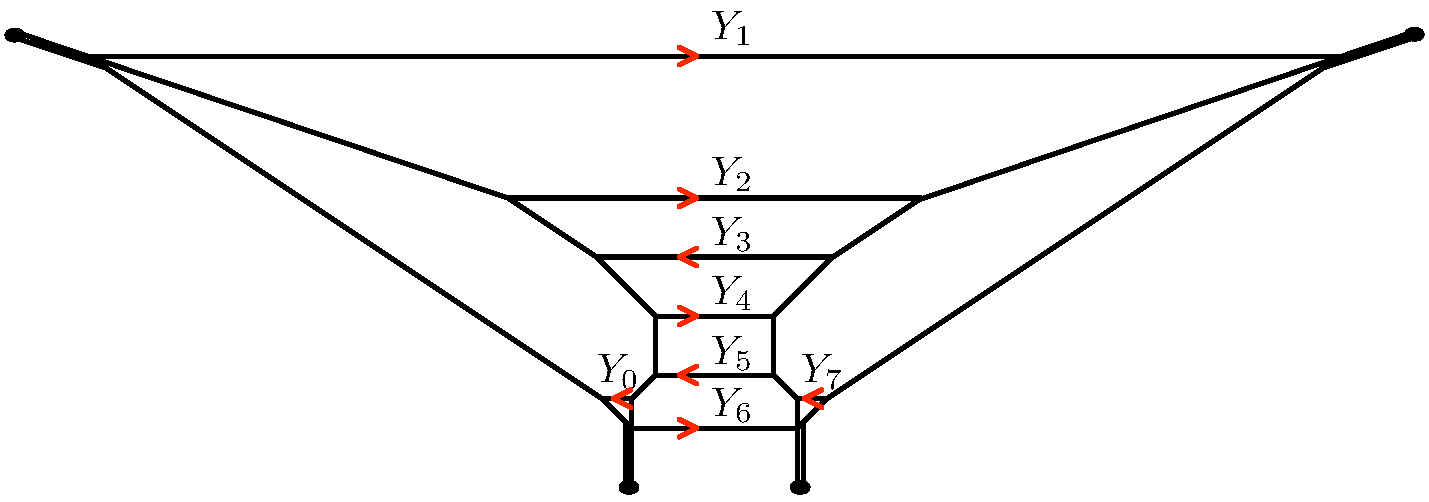
\includegraphics[width=12cm]{SU6young.pdf}
\caption{A labeling of Young diagrams assigned to the horizontal edges of Figure \ref{fig:SU6-monopole}.}
\label{fig:SU6young}
\end{figure}
%----------------------------------%
To compute the instanton partition function based on the 5-brane web for $SU(6)+1{\bf TAS}$ given in Figure \ref{fig:SU6-monopole}, we assign the Young diagrams $Y_i$ to each horizontal edge of the web diagram as shown in Figure \ref{fig:SU6young} and use the topological vertex method. For convenience, we restrict to ourselves to the unrefined case where $2\epsilon_+=\epsilon_1+\epsilon_2=0$. (See also a similar calculation done in \cite{Hayashi:2019yxj}.) As the web diagram in Figure \ref{fig:SU6-monopole} is left-right symmetric, it is convenient to split the web diagram as the left and right part and glue to obtain the partition function. With the K\"ahler parameters for Coulomb branch moduli $A_i, (i=1, \cdots, 6)$ subject to $\prod_{i=1}^{6}A_i =1$, the instanton $q$, and the unrefined $\Omega$-deformation parameter $g$, defined by 
\begin{align}
A_i = e^{-a_i}
%\quad \Big(\prod_{i=1}^{6}A_i =1\Big)\, 
, \qquad q = e^{-\frac{8\pi^2}{g_0^2}}% = e^{-4\pi^2m_0}
, \qquad g=e^{-\epsilon_-},
\end{align}
one finds that 
\begin{align}
  \label{eq:znek-su6}
  Z_{\text{Nek}} 
  =&\, \sum_{(Y_1, \cdots, Y_6)}q^{\sum_{i=1}^6|Y_i|} (-A_1^6)^{|Y_1|}(-A_2^6)^{|Y_2|}(-A_2^2A_3^4)^{|Y_3|}(-A_2^2A_3^2A_4^2)^{|Y_4| + |Y_5|}\nn\\
  &\times f_{Y_1}(g)^5f_{Y_2}(g)^5f_{Y_3}(g)^3f_{Y_4}(g)f_{Y_5}(g)^{-1}f_{Y_6}(g)^{2}
  Z_{\text{left}}(\vec{Y})Z_{\text{right}}(\vec{Y}),
%  Z_{\text{half}}\,(Y_1, Y_2, Y_3, Y_4, Y_5, Y_6)^2. 
\end{align}
%\begin{align}
%Z_{\text{Nek}} 
%=&\, \sum_{\vec{Y}}q^{\sum_{i=1}^6|Y_i|} (-A_1^6)^{|Y_1|}(-A_2^6)^{|Y_2|}(-A_2^2A_3^2A_4^2)^{|Y_3|}(-A_2^2A_3^4)^{|Y_4| + |Y_5|}\nn\\
%&\times f_{Y_1}(g)^5f_{Y_2}(g)^5f_{Y_3}(g)^3f_{Y_4}(g)f_{Y_5}(g)^{-1}f_{Y_6}(g)^{2}Z_{\text{left}}(\vec{Y})Z_{\text{right}}(\vec{Y}), \label{Znek1}
%\end{align}
where $\vec{Y}=(Y_1, Y_2, Y_3, Y_4, Y_5, Y_6)$ and the left and right parts,
$Z_{\text{left}}(\vec{Y})$ and $Z_{\text{right}}(\vec{Y})$, are given by
\begin{align}
Z_{\text{left}}(\vec{Y})=& \,
\sum_{Y_0} ( - A_1{}^{-1} A_6{}^{-2})^{|Y_0|} 
g^{\frac{||Y_0^t||^2+||Y_0||^2}{2}} \tilde{Z}_{Y_0}^2 f_{Y_0}^2(g)
\prod_{i=1}^6 g^{\frac{||Y_i||^2}{2}} \tilde{Z}_{Y_i} 
\cr 
& 
\times 
R_{Y_1 Y_6^t}^{-1} (A_1 A_6{}^{-1})\,R_{Y_0 Y_6^t}^{-1} (A_1{}^{-1} A_6{}^{-2})\,R_{Y_1Y_0^t }^{-1} (A_1^2A_6) \cr 
& 
\times  
 \prod_{2 \le i <  j \le 5} R_{Y_i Y_j^t}^{-1} (A_i A_j{}^{-1})
 \prod_{i=2}^5 R_{Y_0^t Y_i} (A_1 A_i  A_6) ,
\end{align}
and $Z_{\text{right}}(\vec{Y})$ is obtained from $Z_{\text{left}}(\vec{Y})$ by replacing $Y_0$ with $Y_7$. % summing over $Y_7$ instead of $Y_0$. %  \big|_{Y_0 \to Y_7}$.
%\begin{align}
%Z_{\text{right}}(\vec{Y})=&
%\sum_{Y_7} ( - A_1{}^{-1} A_6{}^{-2})^{|Y_7|} 
%g^{\frac{||Y_7^t||^2+||Y_7||^2}{2}} \tilde{Z}_{Y_7}^2 f_{Y_7}^2(g)
%\prod_{i=1}^6 g^{\frac{||Y_i||^2}{2}} \tilde{Z}_{Y_i} 
%\cr 
%& 
%%\times 
%%R_{Y_1 Y_6^t}^{-1} (A_1 A_6{}^{-1}) \prod_{2 \le i <  j \le 5} R_{Y_i Y_j^t}^{-1} (A_i A_j{}^{-1})
%%\cr 
%%& 
%%\times  
%%R_{Y_7 Y_6^t} (A_1{}^{-1} A_6{}^{-2})\prod_{i=1}^5 R_{Y_7^t Y_i} (A_1 A_i  A_6).
%\times 
%R_{Y_1 Y_6^t}^{-1} (A_1 A_6{}^{-1})\,R_{Y_7 Y_6^t}^{-1} (A_1{}^{-1} A_6{}^{-2})\,R_{Y_1Y_7^t }^{-1} (A_1^2A_6) \cr 
%& 
%\times  
% \prod_{2 \le i <  j \le 5} R_{Y_i Y_j^t}^{-1} (A_i A_j{}^{-1})
% \prod_{i=2}^5 R_{Y_7^t Y_i} (A_1 A_i  A_6) .
%\end{align}
Here, for a Young diagram $\lambda = (\lambda_1, \lambda_2, \cdots)$ and its transpose $\lambda^t$,  $|\lambda|=\sum_{i}\lambda_i$ and $||\lambda||^2 =\sum_{i}\lambda_i^2$ and 
\begin{align}
\tilde{Z}_{\lambda} 
&= \prod_{(i,j) \in \lambda} \frac{1}{1 - g^{\lambda_i + \lambda^t_j - i - j +1} }. 	
\end{align}
The framing factor $f_{\lambda}(g)$ is defined by
\begin{align}
f_\lambda(g) = (-1)^{|\lambda|}g^{\frac{1}{2}(g^{||\lambda^t||^2 - ||\lambda||^2})},
\end{align}
and $R_{\lambda \mu } (Q)=R_{\mu \lambda} (Q)$ is defined by
\begin{align}
%\tilde{Z}_{\lambda} 
%&= \prod_{(i,j) \in \lambda} \frac{1}{1 - g^{\lambda_i + \lambda^t_j - i - j +1} } , 
%\cr
R_{\lambda \mu } (Q)%= \prod_{i.j=1}^{\infty} (1 - Q g^{i+j-\lambda_j - \mu_i -1}),\cr
=\text{PE} \left[ - \frac{g}{(1-g)^2} Q \right]
\times N_{\lambda^t \mu} (Q)
\end{align}
with PE representing the Plethystic exponential
 and 
\begin{align}
N_{\lambda \mu} (Q) 
= \prod_{(i,j) \in \lambda} \left( 1 - Q g^{\lambda_i + \mu_j^t -i-j+1} \right)
\prod_{(i,j) \in \mu} \left( 1 - Q g^{-\lambda^t_j - \mu_i + i + j - 1} \right). 
\end{align}
%and $f_{\lambda}(g)$ is the framing factor defined by
%\begin{align}
%f_\lambda(g) = (-1)^{|\lambda|}g^{\frac{1}{2}(g^{||\lambda^t||^2 - ||\lambda||^2})},
%\end{align}
%with $|\lambda|=\sum_{i}\lambda_i$ and $||\lambda||^2 =\sum_{i}\lambda_i^2$ for a Young diagram $\lambda = (\lambda_1, \lambda_2, \cdots)$ and its transpose $\lambda^t$. %=(\lambda^t_1, \lambda^t_2, \cdots)$ .
%Moreover, $A_i, (i=1, \cdots, 6)$, $q$ and $g$ are defined by 
%and the Coulomb branch parameters $A_i, (i=1, \cdots, 6)$, the instanton fugacity $q$ and the unrefined $\Omega$-deformation parameter $g$ are defined by 
%\begin{align}
%A_i = e^{-a_i}, \qquad q = e^{-m_0}, \qquad g=e^{-\epsilon}.
%\end{align}
The Nekrasov partition function is then expressed as a weighted sum of the instanton partition function %of the perturbative partition and the weighted sum of $k$-instanton partition functions $Z_k$
\begin{align}
Z_{\text{Nek}} = Z_{\text{pert}}\bigg(1 + \sum_{k=1}^{\infty}q^kZ_k\bigg) ,
\end{align}
where $Z_{\text{pert}}$ is the perturbative partition function, while $Z_k$ stands for the $k$-instanton partition function. 
The perturbative part of the partition function $Z_{\text{pert}}$ comes from the summand of \eqref{eq:znek-su6} at empty Young diagrams, i.e., %$(Y_1, Y_2, Y_3, Y_4, Y_5, Y_6) = (\varnothing,\varnothing,\varnothing,\varnothing,\varnothing,\varnothing)$. 
$(Y_1, Y_2, Y_3, Y_4, Y_5, Y_6) = (\o,\o,\o,\o,\o,\o)$
It is given by
\begin{align}
Z_{\rm pert} 
=& \,
Z_{\text{left}}(\o,\o,\o,\o,\o,\o)
Z_{\text{right}}(\o,\o,\o,\o,\o,\o)
\cr
=&\, 
\text{PE} \Biggl[ 
\frac{2g}{(1-g)^2} 
\Bigl( \frac{A_1}{A_6} + \frac{1}{A_1A_6^2} + A_1^2  A_6 
+ \sum_{2 \le i <  j \le 5} \frac{A_i}{A_j}
- \sum_{i=2}^5 A_1 A_i  A_6
\Bigr)
\Biggr]
\cr 
& 
\times \bigg(\sum_{Y_0} ( - A_1{}^{-1} A_6{}^{-2})^{|Y_0|} \ 
g^{\frac{\Vert Y_0^t \Vert ^2+\Vert Y_0\Vert ^2}{2}} \tilde{Z}_{Y_0}(g)^2 f_{Y_0}^2(g)
\cr 
& \qquad \qquad
\textstyle N_{Y_0^t \,\o }^{-1} (A_1{}^{-1} A_6{}^{-2})
 N^{-1}_{Y_0 \,\o } (A_1^2  A_6)\prod_{i=2}^5 N_{Y_0 \,\o } (A_1 A_i  A_6)\bigg)^2 ,\label{eq:zpert-top}
\end{align}
%\begin{align}
%  \label{eq:zpert-top}
%Z_{\rm pert} 
%=& \,
%Z_{\text{half}}(\varnothing,\varnothing,\varnothing,\varnothing,\varnothing,\varnothing)^2
%\cr
%=&\, 
%\text{PE} \Biggl[ 
%\frac{2g}{(1-g)^2} 
%\Bigl( \frac{A_1}{A_6} + \frac{1}{A_1A_6^2} + A_1^2  A_6 
%+ \sum_{2 \le i <  j \le 5} \frac{A_i}{A_j}
%- \sum_{i=2}^5 A_1 A_i  A_6
%\Bigr)
%\Biggr]
%\cr 
%& 
%\times \bigg(\sum_{Y_0} ( - A_1{}^{-1} A_6{}^{-2})^{|Y_0|} \ 
%g^{\frac{\Vert Y_0^t \Vert ^2+\Vert Y_0\Vert ^2}{2}} \tilde{Z}_{Y_0}(g)^2 f_{Y_0}^2(g)
%\cr 
%& \qquad \qquad
%\textstyle N_{Y_0^t \varnothing }^{-1} (A_1{}^{-1} A_6{}^{-2})
% N^{-1}_{Y_0 \varnothing } (A_1^2  A_6)\prod_{i=2}^5 N_{Y_0 \varnothing } (A_1 A_i  A_6)\bigg)^2 ,
%\end{align}
where the last two lines can be  combined into the following closed-form expression:
\begin{align}
  \text{PE} \Biggl[ 
    \frac{2g}{(1-g)^2} 
    \Bigl(\sum_{i=2}^5  \frac{A_1}{A_i} +\sum_{i=2}^5  \frac{A_i}{A_6} - \frac{1}{A_1A_6^2} - A_1^2  A_6 
    - \sum_{2\leq i<j \leq 5} A_1 A_i  A_j + \mathcal{O}(A_1^6)
    \Bigr)
    \Biggr].
\end{align}
We note here that when performing the Young diagram sum over $Y_0$ in \eqref{eq:zpert-top} to compute the $Z_{\rm pert}$, we expand \eqref{eq:zpert-top} in terms of $A_1$ and, by $\mathcal{O}(A_1^6)$, we mean that the obtained result is valid up to $\mathcal{O}(A_1^6)$. As it is very unlikely that there will be a new term which suddenly appears  in higher orders than 6 in $A_1$, we believe that there are no further terms for $\mathcal{O}(A_1^6)$.  
It is clear then that \eqref{eq:zpert-top} is manifestly consistent with the equivariant index  \cite{Shadchin:2005mx} for 5d $SU(6)$ gauge theory with a hypermultiplet in the rank-3 antisymmetric representation, %$\mathbf{20}$, 
i.e., 
\begin{align}
  Z_{\rm pert}  = \text{PE} \Biggl[ 
    \frac{2g}{(1-g)^2} 
    \Bigl(\sum_{1\leq i<j \leq 6}  \frac{A_i}{A_j} 
    - \sum_{2\leq i<j \leq 6} A_1 A_i  A_j %+ \mathcal{O}(A_1^6)
    \Bigr)
    \Biggr].
\end{align}
The 1-instanton partition function $Z_1$ can be obtained from the summands of \eqref{eq:znek-su6} at Young diagrams satisfying $\sum_{i=1}^6 |Y_i|=1$. There are 6 different profiles of Young diagrams. The configuration $|Y_i| = 1$ and %$Y_{j\neq i} = \varnothing$
$Y_{j\neq i} = \o$ contribute to $Z_{1}$ as
\begin{align}
  + \frac{g}{(1-g)^2} \frac{A_i^6}{\prod_{j \neq i} (A_i - A_j)^2} 
  \Bigl(-A_i \sum_{j\neq i} A_j +  \sum_{j\neq i}\frac{1}{A_j}  - \frac{1}{A_i} + A_i^2
 \Bigr)^2. 
\end{align}
Summing over all six contributions, one finds
\begin{align}
  Z_1 = \sum_{i=1}^6 \frac{g}{(1-g)^2} \frac{A_i^6}{\prod_{j \neq i} (A_i - A_j)^2} 
  \Bigl(-A_i \sum_{j\neq i} A_j +  \sum_{j\neq i}\frac{1}{A_j}  - \frac{1}{A_i} + A_i^2
 \Bigr)^2. 
\end{align}
which is in agreement with the blowup partition function (eqn). \textcolor{red}{(overall sign: looking at the GV invariant for single W-boson + single instanton (which should be -2), the topological vertex computation seems to be correct. blowup should have an overall sign issue)}